\title{Parallel Programming Assignment 1: Game of Life}
\author{
        %\large
        \textsc{Caitlin Ross}
  %          \qquad
     %   \textsc{}
        \mbox{}\\ %
        Department of Computer Science\\
        CSCI 6360\\
         \\
        \mbox{}\\ %
        \normalsize
            \texttt{rossc3}
     %   \textbar{}
        %    \texttt{yogi}
        \normalsize
            \texttt{@rpi.edu}
}
\date{\today}
\documentclass[11pt]{article}
%\documentclass{acmconf}

\usepackage[paper=a4paper,dvips,top=1.5cm,left=1.5cm,right=1.5cm,
    foot=1cm,bottom=1.5cm]{geometry}

\usepackage{times}
%\usepackage{graphicx}
\usepackage[fleqn]{amsmath}
\usepackage{amsfonts}
\usepackage{amssymb}
\usepackage{amsthm}
\usepackage{amsopn}
\usepackage{xspace}
\usepackage{array}
\usepackage{epsfig}

\numberwithin{figure}{section}

\newcommand\CC{\Lang{\mbox{C++}}\xspace}
\newcommand\Lang[1]{\textsc{#1}}
\newcommand{\kw}[1]{\texttt{\textbf{#1}}}
\newcommand{\cd}[1]{\texttt{#1}}

\newcommand\Naturals{\ensuremath{\mathbb{N}}\xspace}
\newcommand\Integers{\ensuremath{\mathbb{Z}}\xspace}
\newcommand\Rationals{\ensuremath{\mathbb{Q}}\xspace}
\newcommand\Reals{\ensuremath{\mathbb{R}}\xspace}
\newcommand\Complex{\ensuremath{\mathbb{C}}\xspace}

\newcommand\norm[1]{\ensuremath{\lVert#1\rVert}}
\newcommand\abs[1]{\ensuremath{\lvert#1\rvert}}
\newcommand\ceil[1]{\ensuremath{\lceil#1\rceil}}
\newcommand\floor[1]{\ensuremath{\lfloor#1\rfloor}}
\newcommand\set[1]{\ensuremath{\{#1\}}}
\newcommand\angular[1]{\ensuremath{\langle#1\rangle}}

\newcommand\Norm[1]{\ensuremath{\left\lVert#1\right\rVert}}
\newcommand\Abs[1]{\ensuremath{\left\lvert#1\right\rvert}}
\newcommand\Ceil[1]{\ensuremath{\left\lceil#1\right\rceil}}
\newcommand\Floor[1]{\ensuremath{\left\lfloor#1\right\rfloor}}
\newcommand\Set[1]{\ensuremath{\left\{#1\right\}}}
\newcommand\Angular[1]{\ensuremath{\left\langle#1\right\rangle}}

\newcommand{\LOOM}{\ensuremath{\cal{LOOM}}\xspace}
\newcommand{\PolyTOIL}{\textbf{PolyTOIL}\xspace}

\newtheorem{theorem}{Theorem}[section]
\newtheorem{definition}[theorem]{Definition}
\newtheorem{lemma}[theorem]{Lemma}
\newtheorem{corollary}[theorem]{Corollary}
\newtheorem{fact}[theorem]{Fact}
\newtheorem{example}[theorem]{Example}

\newcommand\Cls[1]{\textsf{#1}}
\newcommand\Fig[1]{Figure~\ref{Figure:#1}}

\usepackage{labels} %
%\usepackage{equation}
%\usepackage{prog2tex}

\newenvironment{excerpt}{\begin{quote}\begin{minipage}\textwidth}{\end{minipage}\end{quote}}

\setcounter{topnumber}{0}
\setcounter{bottomnumber}{0}
\setcounter{totalnumber}{20}
\renewcommand{\textfraction}{0.01}

\begin{document}
\newgeometry{margin=1in}

\maketitle

\section{Game of Life}
This assignment is to implement a Game of Life program.  There is a 2D grid of square cells, where each cell is either ALIVE or DEAD.  Each cell interacts with its eight neighbors according to a set of rules.  If a live cell has less than two living neighbors, it dies. If a live cell has two or three living neighbors, it lives.  Otherwise if a live cell has more than 3 living neighbors, it dies.  If a dead cell has three living neighbors, the dead cell becomes a living cell.  

In each generation or ``tick,'' these rules are applied to each cell in the grid.  The experiments performed for this assignment are on a 16x16 cell universe with 100 ticks.  Some additional randomness is added into the previously described rules.  For a given threshold, if a random number is greater than the threshold, then the basic rules are applied.  Otherwise a state is randomly chosen for that cell.  The experiments are performed with thresholds of 0\%, 25\%, 50\%, 75\%, and 90\%.  

\section{Results}
In all figures, cells that are ALIVE are represented as a yellow block, while DEAD cells are black.  Figure \ref{fig:0} shows the results where the threshold is 0\%.  In this situation, the rules are always applied to every cell in each generation.  The pattern here tends towards longer lines of live cells, with large chunks of dead cells.  Figure \ref{fig:25} is where randomness starts to affect the state of the game.  There is a 25\% chance of a cell's state being randomly selected, so we don't see as many long lines of living cells as the previous graph.  Figures \ref{fig:50}, \ref{fig:75}, and \ref{fig:90} have thresholds of 50\%, 75\%, and 90\% respectively.  As the threshold gets larger, randomness has a greater effect on the system and there is less of a noticeable pattern in the graphs.  

\begin{figure}[t]
\centering
   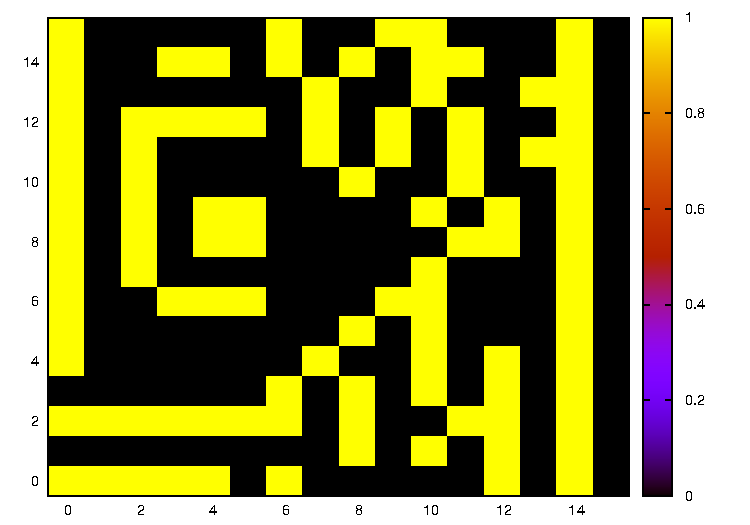
\includegraphics{gol-16-100-0.pdf}
\caption{Final state for 16x16 universe, 100 ticks and threshold 0\%}
\label{fig:0}
\end{figure}
\begin{figure}[t]
\centering
   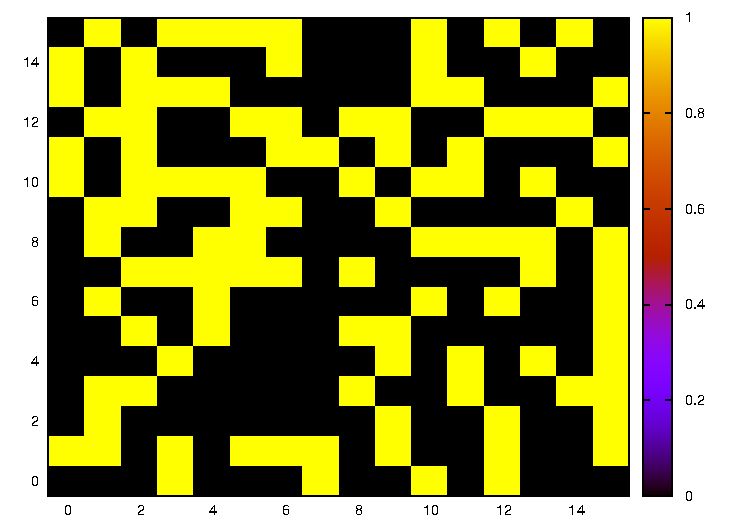
\includegraphics{gol-16-100-25.pdf}
\caption{Final state for 16x16 universe, 100 ticks and threshold 25\%}
\label{fig:25}
\end{figure}
\begin{figure}[t]
\centering
   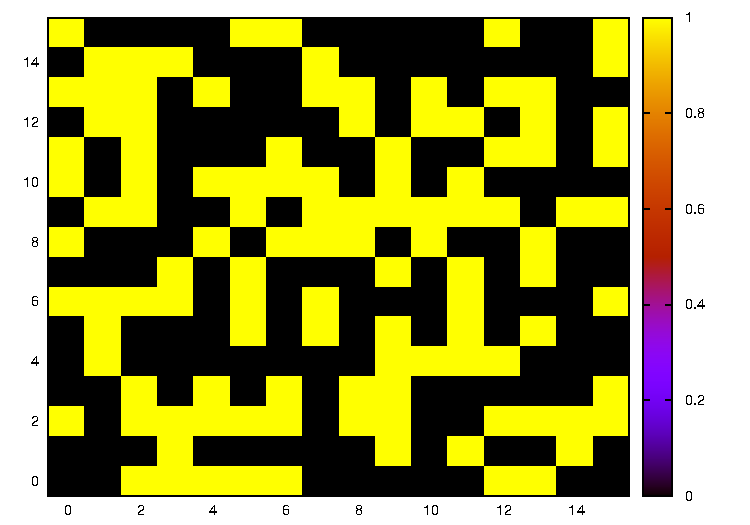
\includegraphics{gol-16-100-50.pdf}
\caption{Final state for 16x16 universe, 100 ticks and threshold 50\%}
\label{fig:50}
\end{figure}
\begin{figure}[t]
\centering
   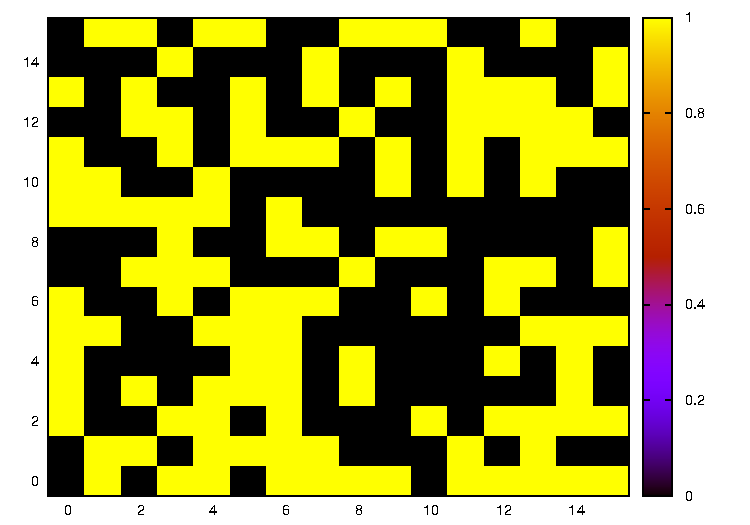
\includegraphics{gol-16-100-75.pdf}
\caption{Final state for 16x16 universe, 100 ticks and threshold 75\%}
\label{fig:75}
\end{figure}
\begin{figure}[t]
\centering
   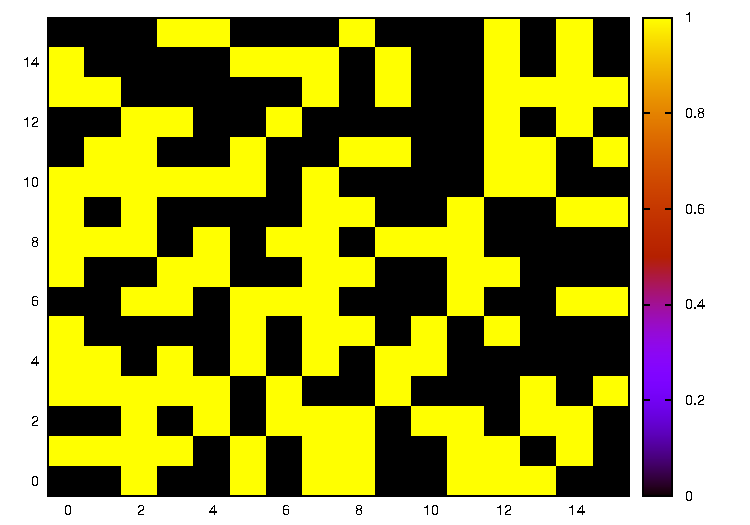
\includegraphics{gol-16-100-90.pdf}
\caption{Final state for 16x16 universe, 100 ticks and threshold 90\%}
\label{fig:90}
\end{figure}






%\bibliography{main}

%\bibliographystyle{abbrv}
\end{document}
